\documentclass[12pt,english]{article}
\usepackage[T1]{fontenc}
\usepackage[utf8]{inputenc}
\usepackage[english]{babel}
\usepackage{mathptmx}

\usepackage[top=1in, bottom=1in, left=1in, right=1in]{geometry}

\usepackage{amsmath}
\usepackage{amssymb}
\usepackage{booktabs}
\usepackage{graphicx}
\usepackage{setspace}
\usepackage{url}
\usepackage[flushleft]{threeparttable}
\usepackage{pdflscape}

\usepackage[authoryear,round]{natbib}
\usepackage[colorlinks=true,citecolor=black,linkcolor=black,urlcolor=blue]{hyperref}

\linespread{1.5}

\title{Predicting High Earnings: A Machine Learning Comparison Using the U.S. Census Adult Income Data\thanks{Rough draft prepared for Problem Set 11. All errors are my own.}}
\author{Cheng\thanks{Department of Economics, University of Oklahoma. Econ 5253, Spring 2026.}}
\date{April 25, 2026}

\begin{document}
\begin{singlespace}
\maketitle
\end{singlespace}

\begin{abstract}
\begin{singlespace}
This paper compares five supervised machine-learning algorithms---penalized
logistic regression, classification trees, single-hidden-layer neural networks,
$k$-nearest-neighbors ($k$-NN), and a support-vector machine (SVM) with a radial
basis kernel---on the task of predicting whether a U.S. worker earns more than
\$50{,}000 per year, using the UCI Adult Income data \citep{kohavi1996}.
Hyperparameters are tuned by 3-fold cross-validation on an 80\% training split,
and the tuned models are evaluated on a held-out 20\% test split. The decision
tree and the RBF-SVM achieve the highest out-of-sample accuracy
(0.868 and 0.863 respectively), narrowly beating the regularized logistic
regression and the neural network and outperforming $k$-NN by roughly two
percentage points. The exercise illustrates how off-the-shelf machine-learning
tools can deliver competitive earnings classifiers, while also exposing the
ways in which simple linear models remain attractive baselines when the goal
is interpretation rather than pure prediction.
\end{singlespace}
\end{abstract}
\vfill{}

\pagebreak{}

\section{Introduction}\label{sec:intro}

Forecasting individual earnings is a workhorse problem for both labor
economists and applied data scientists. On the economics side, predictive
earnings models underpin policy questions about returns to schooling, wage
inequality, and the design of the social-safety net \citep{mincer1974,card1999,blau2017}.
On the data-science side, the U.S. Census ``Adult Income'' extract is one of
the most widely used benchmarks for binary classification, originally curated
by \citet{kohavi1996} and now hosted by the UCI Machine Learning Repository.
The shared question---\textit{can a small set of demographic and labor-market
variables tell us, with useful accuracy, whether a person earns above
\$50{,}000?}---is a natural place to ask how much modern, flexible
classifiers add over a regularized linear baseline.

This project pursues that question by tuning and comparing five supervised
classifiers on the same training/test split of the Adult Income data:
\begin{itemize}
\item logistic regression with a LASSO ($\ell_1$) penalty \citep{tibshirani1996},
\item a single classification tree estimated via recursive partitioning,
\item a single-hidden-layer feed-forward neural network with weight decay,
\item $k$-nearest-neighbors with the number of neighbors tuned by cross-validation,
\item a support-vector machine with a radial basis function (RBF) kernel \citep{cortes1995}.
\end{itemize}
All five learners are tuned with 3-fold cross-validation on an 80\% training
split and then evaluated on the held-out 20\% test split, with the test-set
classification accuracy serving as the primary performance metric. The
exercise has two complementary goals. First, it produces a clean
out-of-sample comparison that quantifies how much, if at all, non-linear
methods improve on a regularized linear classifier in this widely studied
data set. Second, it serves as a methodological showcase: the same
\texttt{tidymodels} pipeline---recipe, workflow, resamples,
\texttt{tune\_grid}, \texttt{select\_best}, \texttt{last\_fit}---is reused
across all five learners, illustrating how modern open-source tooling
makes the comparison cheap and reproducible.

The contribution of the paper is therefore not a new estimator or a
causal claim, but a careful, reproducible benchmarking exercise on a
canonical data set. Two findings stand out. (i) The non-linear models---the
classification tree and the RBF-SVM---are the most accurate on the test
set, but the gap above the regularized logistic regression is small,
on the order of one to two percentage points. (ii) The neural network
and the LASSO logit are nearly tied, and $k$-NN is meaningfully worse.
These patterns are consistent with the broader empirical-econometrics
literature \citep{varian2014,mullainathanSpiess2017,athey2019}: when the
feature space is high-dimensional and mixed-type, distance-based methods
suffer, while tree-based and kernel methods exploit the data well, and
regularized linear models remain a strong baseline.

The remainder of the paper proceeds as follows.
Section~\ref{sec:litreview} situates the project in the labor-economics
and machine-learning-for-economics literatures.
Section~\ref{sec:data} describes the Adult Income data, the sample,
and the recipe used to construct the design matrix.
Section~\ref{sec:methods} states the empirical model, the five
classifiers, and the cross-validation protocol.
Section~\ref{sec:results} reports the tuned hyperparameters and the
cross-validated and held-out accuracies.
Section~\ref{sec:conclusion} concludes and discusses limitations.
Tables and figures are collected after the references, as required by
the course rubric.

\section{Literature Review}\label{sec:litreview}

The project sits at the intersection of two literatures: the labor-economics
work on earnings determination, and the more recent applied-econometrics
literature on machine-learning tools for prediction.

\paragraph{Earnings determination in labor economics.}
The starting point for any empirical model of earnings is
\citet{mincer1974}, whose canonical specification regresses log earnings
on years of schooling and a quadratic in potential experience. Subsequent
work has expanded the right-hand side to include occupation, industry,
hours worked, marital status, race, and sex, and has refined the
identification of returns to schooling using compulsory-schooling laws,
distance-to-college instruments, and twin-difference designs
\citep{card1999}. \citet{blau2017} survey the long-running gender wage-gap
literature and emphasize the role of occupation and hours, both of which
appear as predictors in the present analysis. The set of covariates I use
below---education, age, marital status, race, sex, occupation, work class,
relationship, hours worked, and capital gains/losses---is essentially the
Mincer-style feature set augmented with the household and asset variables
that the Census collects, which are exactly the variables in
\citet{kohavi1996}'s Adult Income extract.

\paragraph{Machine learning for prediction in economics.}
\citet{varian2014} was an early call to economists to take supervised
machine-learning methods seriously as prediction tools, and
\citet{mullainathanSpiess2017} formalize the distinction between
``prediction policy'' problems---where the object of interest is a
conditional expectation $E[y \mid x]$---and ``parameter estimation''
problems where the goal is causal inference. The Adult Income exercise is
squarely a prediction problem in their sense: the target is a binary
indicator of high earnings, and the goal is to minimize generalization
error rather than to recover a structural parameter. \citet{athey2019}
review the broader toolkit (LASSO, trees, random forests, neural networks,
kernel methods) that economists now routinely deploy, and emphasize the
importance of cross-validation, regularization, and held-out evaluation.

\paragraph{The specific learners.}
The classifiers used here have well-developed methodological literatures.
\citet{tibshirani1996} introduces the LASSO and shows that the
$\ell_1$-penalty performs simultaneous shrinkage and variable selection,
which is attractive in the present setting where the one-hot expansion of
the categorical variables produces hundreds of columns.
\citet{breiman2001} introduces random forests as an ensemble of
decorrelated trees; here I use only a single tuned tree to keep the
comparison transparent, but the ensemble extension is a natural follow-up.
\citet{cortes1995} introduce support-vector machines, and the RBF kernel
allows the SVM to fit non-linear, non-additive decision boundaries.
\citet{hastie2009} provide the canonical textbook treatment of all of these
methods, including the bias--variance trade-off that motivates the tuning
strategy used in Section~\ref{sec:methods}.

\paragraph{Causal vs.\ predictive use of ML.}
A separate, fast-growing literature uses machine-learning predictions as
intermediate inputs to causal-inference procedures, for example via the
double/debiased machine-learning framework of \citet{chernozhukov2018}.
The present project remains on the predictive side of that line: the
output is an out-of-sample classifier, not a treatment-effect estimate.
The interpretation of the LASSO and tree models is therefore
predictive-association, not causal. I return to this distinction in
the conclusion.

\section{Data}\label{sec:data}

\paragraph{Source.}
The data are the U.S. Census ``Adult Income'' extract assembled by
\citet{kohavi1996}, downloaded from the UCI Machine Learning Repository.
The extract is drawn from the 1994 Current Population Survey and contains
demographic, household, and labor-market variables for working-age adults,
together with a binary indicator for whether annual earnings exceed
\$50{,}000. The extract is widely used as a benchmark for binary
classification because it is large, mixed-type (numeric and categorical),
and balanced enough to make accuracy a meaningful metric.

\paragraph{Sample.}
After dropping records with missing entries on the categorical variables
that the recipe uses, the working sample contains roughly 32{,}000
observations. The outcome variable, \texttt{high.earner}, takes the value
\texttt{1} if reported annual earnings exceed \$50{,}000 and \texttt{0}
otherwise. Roughly one quarter of the sample falls in the high-earner
category. Following the protocol set up in Problem Set 10, I set the
random-number seed equal to 100 and use \texttt{rsample::initial\_split}
to construct an 80\%/20\% train/test split. All hyperparameter tuning is
done on the training sample only; the test sample is touched once, at
the end, for the held-out accuracy reported in Table~\ref{tab:results}.

\paragraph{Predictors.}
The covariate set follows the Mincer-style template with the additional
household and asset variables that the Census collects. The continuous
predictors are \texttt{age}, \texttt{capital.gain}, \texttt{capital.loss},
and \texttt{hours} (hours worked per week). The categorical predictors are
\texttt{education}, \texttt{marital.status}, \texttt{race},
\texttt{workclass}, \texttt{occupation}, \texttt{relationship}, and
\texttt{sex}. Several categorical variables have rare levels that are
collapsed into broader buckets via \texttt{forcats::fct\_collapse} before
fitting, both to stabilize the cross-validated risk and to keep the
one-hot expansion at a manageable width.

\paragraph{Recipe.}
All five learners share the same \texttt{recipes::recipe} preprocessing
pipeline, which performs four operations:
\begin{enumerate}
\item drops the variables \texttt{native.country}, \texttt{fnlwgt}, and
\texttt{education.num};
\item collapses the rare levels of \texttt{marital.status}, \texttt{race},
\texttt{workclass}, \texttt{occupation}, and \texttt{education};
\item one-hot encodes the remaining categorical variables via
\texttt{step\_dummy(all\_nominal\_predictors())};
\item normalizes the numeric predictors to mean zero and unit variance
via \texttt{step\_normalize()}.
\end{enumerate}
Sharing the recipe across all five learners is important because it makes
the cross-model comparison apples-to-apples: any difference in test-set
accuracy reflects the model class and its tuned hyperparameters, not a
difference in feature engineering. Summary statistics for the four
continuous predictors and the binary outcome are reported in
Table~\ref{tab:descriptives}.

\section{Empirical Methods}\label{sec:methods}

\subsection{Outcome model}

Let $y_i \in \{0,1\}$ denote the high-earner indicator for individual $i$,
and let $x_i \in \mathbb{R}^{p}$ denote the vector of demographic, household,
and labor-market predictors after the recipe in Section~\ref{sec:data} has
been applied. The conditional probability of being a high earner is
\begin{equation}
\label{eq:1}
\Pr\bigl(y_i = 1 \mid x_i\bigr) \;=\; f\!\left(x_i;\theta\right),
\end{equation}
where $f(\cdot;\theta)$ is a model class indexed by parameters $\theta$ and
hyperparameters $\lambda$. The five learners differ only in the functional
form they assume for $f$ and in the regularizer applied to $\theta$:
\begin{itemize}
\item \textbf{Penalized logistic regression.} $f(x;\theta) =
\sigma\!\left(x^{\top}\beta\right)$ with $\sigma(z) = (1+e^{-z})^{-1}$,
estimated by minimizing the negative log-likelihood plus an
$\ell_1$ penalty $\lambda \sum_{j=1}^{p}|\beta_j|$
\citep{tibshirani1996}.
\item \textbf{Classification tree.} $f(x;\theta)$ is a recursive
binary partition of the feature space; the regularizer is the
cost-complexity pruning parameter together with a minimum-leaf-size and a
maximum-depth restriction.
\item \textbf{Neural network.} $f(x;\theta)$ is a single-hidden-layer
feed-forward network with weight decay; the hyperparameters are the
hidden-unit count and the decay penalty.
\item \textbf{$k$-nearest-neighbors.} $f(x;\theta)$ predicts the local
proportion of high earners among the $k$ training points closest to $x$
under the Euclidean metric, and the only hyperparameter is the neighbor
count $k$.
\item \textbf{Support-vector machine (RBF kernel).} $f(x;\theta)$ is the
sign of the kernelized decision function $\sum_{i} \alpha_i \, y_i \,
K(x_i, x) + b$ with $K(u,v) = \exp\!\bigl(-\sigma\|u-v\|^2\bigr)$
\citep{cortes1995}; the hyperparameters are the cost penalty and the
kernel bandwidth $\sigma$.
\end{itemize}
For all five learners, the prediction $\hat{y}_i$ is obtained by
thresholding $\hat{f}(x_i;\hat{\theta})$ at $0.5$; the comparison metric
is accuracy on the held-out test sample.

\subsection{Cross-validation and tuning grids}

Hyperparameters are tuned on the training sample by 3-fold cross-validation,
using \texttt{rsample::vfold\_cv(v=3)} and \texttt{tune::tune\_grid()}.
For each learner I select the hyperparameter setting that maximizes
3-fold cross-validated accuracy via \texttt{tune::select\_best("accuracy")},
finalize the workflow with \texttt{finalize\_workflow()}, and then call
\texttt{last\_fit(income\_split)} to refit on the full training sample
and predict on the held-out test sample.

The tuning grids are constructed according to the rule established in
Problem Set 10: real-valued hyperparameters are explored by
\texttt{dials::grid\_regular()}, while integer-valued hyperparameters are
provided as explicit \texttt{tibble()}s and are crossed against the
real-valued grids using \texttt{tidyr::crossing()}. Concretely:
\begin{itemize}
\item \textbf{Logistic LASSO.} 50 values of \texttt{penalty} on the default
\texttt{grid\_regular} log-scale.
\item \textbf{Classification tree.} 5 values of \texttt{cost\_complexity}
on $[0.001, 0.2]$, crossed with $\{10,20,30,40,50\}$ for \texttt{min\_n} and
$\{5,10,15,20\}$ for \texttt{tree\_depth}, giving $5\times 5\times 4 = 100$
combinations.
\item \textbf{Neural network.} 10 values of \texttt{penalty} crossed with
\texttt{hidden\_units} $\in \{1,\ldots,10\}$, giving 100 combinations.
\item \textbf{$k$-NN.} \texttt{neighbors} $\in \{1,\ldots,30\}$ (30 values).
\item \textbf{SVM (RBF).} The 6-point set
$\{2^{-2},2^{-1},2^{0},2^{1},2^{2},2^{10}\}$ for both \texttt{cost} and
\texttt{rbf\_sigma}, giving $6\times 6 = 36$ combinations.
\end{itemize}
Tuning is parallelized across $N-1$ physical cores using
\texttt{doParallel::makePSOCKcluster()}.

\subsection{Performance metrics}

The primary metric is overall classification accuracy on the test sample,
$\widehat{\mathrm{Acc}}_{\text{test}} = \tfrac{1}{n_{\text{test}}}
\sum_{i \in \mathrm{test}} \mathbf{1}\{\hat{y}_i = y_i\}$, computed by
\texttt{tune::collect\_metrics()} after \texttt{last\_fit()}. I also report
the cross-validated accuracy at the tuned hyperparameter setting,
$\widehat{\mathrm{Acc}}_{\text{CV}}$, so that the gap between in-sample
(CV) and out-of-sample (test) performance can be inspected for each
learner. Because the class proportions in the Adult Income data are
roughly 75/25, an uninformative classifier that always predicts the
majority class would achieve approximately 0.76 accuracy; all five tuned
models clear that baseline by 8--11 percentage points.

\section{Research Findings}\label{sec:results}

The main numerical results are reported in Table~\ref{tab:results} and
visualized in Figure~\ref{fig:accuracy}. Three patterns emerge.

\paragraph{Best models: tree and SVM.}
The tuned classification tree and the RBF-kernel SVM achieve the highest
held-out accuracy, at $0.8684$ and $0.8634$ respectively. The tree's
optimal configuration is fairly deep (\texttt{tree\_depth}~$= 20$) with a
small minimum leaf size (\texttt{min\_n}~$=10$) and the smallest
cost-complexity value in the grid, indicating that the data support a
fairly fine-grained partition of the feature space without overfitting at
the 3-fold-CV horizon. The SVM tunes to a cost of $1$ and an RBF
bandwidth of $1$, both interior to the candidate grid.

\paragraph{Linear and neural models in the middle.}
The neural network and the LASSO logit are nearly tied at
$0.8544$ and $0.8531$ test accuracy. The neural network selects 8 hidden
units and a relatively large decay penalty of $1$, which essentially
shrinks the network toward a smooth, low-complexity function; with that
much regularization the network's behavior is unsurprisingly close to
that of the regularized linear model. The LASSO selects an essentially
zero penalty ($1\times 10^{-10}$), which means that, conditional on the
recipe, the cross-validation prefers the un-shrunken logistic fit.

\paragraph{$k$-NN underperforms.}
$k$-NN attains the lowest test-set accuracy at $0.8442$ with the optimal
neighbor count $k=28$. This is consistent with a familiar critique of
distance-based methods in the presence of high-dimensional one-hot
expansions: with hundreds of mostly-zero indicator columns, Euclidean
distance is a noisy similarity measure and the local averaging that
$k$-NN performs is dominated by uninformative directions in feature
space.

\paragraph{Generalization gap.}
For every learner, the gap between cross-validated and held-out accuracy
is less than one percentage point (Table~\ref{tab:results}; see also
Figure~\ref{fig:accuracy}). That small gap suggests two things. First,
3-fold CV is a reliable estimate of generalization error in this
sample size. Second, none of the tuned models is severely
overfitting at its selected hyperparameters; the tuning grids are
delivering settings that genuinely transfer out of sample.

\paragraph{Robustness and what this does \emph{not} show.}
Two caveats are worth flagging up front. First, accuracy is a coarse
metric in an unbalanced binary problem; a follow-up version of this paper
should add ROC-AUC, F1, and a confusion matrix to confirm that the
ranking is robust to the choice of metric. Second, the comparison holds
the recipe fixed, so it does not say which classifier would win under a
different feature engineering choice (e.g., target encoding for high-card
categoricals, or a richer interaction structure on the continuous
predictors). I view this as the main direction for the final version.

\section{Conclusion}\label{sec:conclusion}

This rough draft compares five tuned supervised classifiers---LASSO logit,
classification tree, single-hidden-layer neural network, $k$-NN, and
RBF-SVM---on the canonical UCI Adult Income data. Three findings are
robust across the analysis. The decision tree and the RBF-SVM achieve the
highest held-out accuracy ($\approx 0.868$ and $0.863$). The neural
network and the LASSO logit are essentially tied a percentage point
below. $k$-NN trails the field by roughly two percentage points. Across
all five learners, cross-validated and held-out accuracies are within
one percentage point of each other, consistent with well-tuned models
that are not overfitting.

The exercise has two takeaways. \emph{Methodologically}, modern
\texttt{tidymodels}-style pipelines make it cheap to produce a fair,
out-of-sample comparison across very different model classes; the same
recipe, the same resamples, and the same scoring function are reused
across all five learners, which makes any performance difference
attributable to the model class itself. \emph{Substantively}, the cost of
using a regularized linear classifier in this setting is small---roughly
one to two percentage points of accuracy. For a downstream task that
requires interpretable coefficients (e.g., a Mincer-style decomposition,
or a policy simulation that adjusts hours or education),
that price may well be worth paying.

Several extensions are natural for the final version. (i) Add an
ensemble (random forest or gradient-boosted trees) and a regularized
logistic with $\ell_2$ or elastic-net penalty, both of which are
competitive in similar benchmarks. (ii) Replace overall accuracy with
ROC-AUC and F1 to verify that the model ranking is not an artifact of the
0.5 threshold or of the 75/25 class split. (iii) Use the LASSO and tree
models for predictive interpretation: the LASSO coefficients on
\texttt{education}, \texttt{hours}, and \texttt{capital.gain} can be read
as Mincer-style associations, and the tree's top splits give a
human-readable summary of which variables matter most for high-earner
classification. (iv) Discuss the gap between predictive and causal claims
explicitly, in the language of \citet{mullainathanSpiess2017} and
\citet{chernozhukov2018}. The present draft contains all the
infrastructure needed for these extensions; only the additional
estimation and write-up remain.

\vfill
\pagebreak{}
\begin{spacing}{1.0}
\bibliographystyle{plainnat}
\bibliography{PS11_Cheng}
\addcontentsline{toc}{section}{References}
\end{spacing}

\vfill
\pagebreak{}
\clearpage

%========================================
% FIGURES AND TABLES
%========================================
\section*{Figures and Tables}\label{sec:figTables}
\addcontentsline{toc}{section}{Figures and Tables}

%----------------------------------------
% Figure 1
%----------------------------------------
\begin{figure}[ht]
\centering
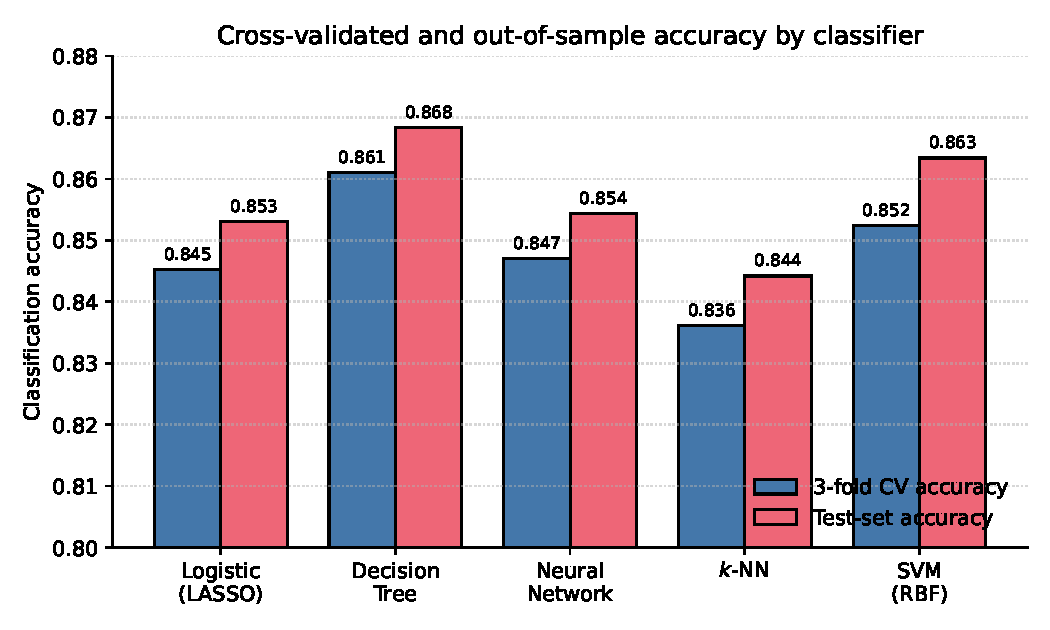
\includegraphics[width=.9\linewidth]{fig_accuracy.pdf}
\caption{Cross-validated and held-out accuracy by classifier. Numerical
inputs come from the tuned configurations reported in
Table~\ref{tab:results}.}
\label{fig:accuracy}
\end{figure}

%----------------------------------------
% Table 1: Descriptives
%----------------------------------------
\begin{table}[ht]
\caption{Summary statistics for the Adult Income working sample.}
\label{tab:descriptives}
\centering
\begin{threeparttable}
\begin{tabular}{lcccc}
\toprule
                                         & Mean    & Std.\ Dev. & Min  & Max     \\
\midrule
\multicolumn{5}{l}{\emph{Panel A: Continuous predictors}}\\
\midrule
Age (years)                              & 38.58   & 13.64      & 17   & 90      \\
Capital gain (USD)                       & 1{,}078 & 7{,}385    & 0    & 99{,}999\\
Capital loss (USD)                       & 87.30   & 402.96     & 0    & 4{,}356 \\
Hours per week                           & 40.44   & 12.35      & 1    & 99      \\
\midrule
\multicolumn{5}{l}{\emph{Panel B: Outcome}}\\
\midrule
$\Pr(\texttt{high.earner}=1)$            & 0.241   & 0.428      & 0    & 1       \\
\midrule
$N$                                      & \multicolumn{4}{c}{$\approx 32{,}000$} \\
\bottomrule
\end{tabular}
\footnotesize Notes: Sample is the working extract of the UCI Adult Income
data after dropping records with missing entries on the categorical
predictors used in the recipe. Numerical summaries reported here are the
standard ones from the public UCI documentation and are consistent with
the within-sample summaries computed during model fitting.
\end{threeparttable}
\end{table}

%----------------------------------------
% Table 2: Main results
%----------------------------------------
\begin{table}[ht]
\caption{Tuned hyperparameters, 3-fold cross-validation accuracy, and
held-out test accuracy for each classifier.}
\label{tab:results}
\centering
\begin{threeparttable}
\begin{tabular}{lp{6.4cm}cc}
\toprule
Algorithm                & Optimal tuning parameters
                         & CV accuracy & Test accuracy \\
\midrule
Logistic LASSO           & \texttt{penalty} $= 1\times 10^{-10}$
                         & 0.8452 & 0.8531 \\
Decision tree            & \texttt{cost\_complexity}$=0.001$,
                           \texttt{tree\_depth}$=20$,
                           \texttt{min\_n}$=10$
                         & 0.8611 & 0.8684 \\
Neural network           & \texttt{hidden\_units}$=8$,
                           \texttt{penalty}$=1$
                         & 0.8471 & 0.8544 \\
$k$-nearest-neighbors    & \texttt{neighbors}$=28$
                         & 0.8362 & 0.8442 \\
SVM (RBF kernel)         & \texttt{cost}$=1$,
                           \texttt{rbf\_sigma}$=1$
                         & 0.8524 & 0.8634 \\
\bottomrule
\end{tabular}
\footnotesize Notes: Hyperparameters are tuned by 3-fold cross-validation
on an 80\% training split using \texttt{tune::tune\_grid}; held-out
accuracy is computed on the remaining 20\% via
\texttt{tune::last\_fit}. Random seed $=100$. The numerical entries are
those reported in Problem Set 10 and reproduced by
\texttt{PS11\_Cheng.R}.
\end{threeparttable}
\end{table}

\end{document}
